% !TEX program = pdflatex
\documentclass[12pt]{article}
\usepackage[reqno]{amsmath}
\usepackage{amssymb,amsthm,graphicx,verbatim,url,verbatim,longtable,vmargin,accents,bbm,times,subfig,dcolumn,booktabs,setspace,soul,latexsym,wasysym,titling,enumitem,longtable,booktabs,xr}
\externaldocument{acc-supp}
\allowdisplaybreaks
% \usepackage{showkeys}

\usepackage[export]{adjustbox}
\usepackage[dvipsnames,usenames]{xcolor}
\definecolor{spot}{rgb}{0.6,0,0}

\usepackage{tikz}\usetikzlibrary{tikzmark,arrows,calc,arrows.meta}
\usepackage[T1]{fontenc}\usepackage[encapsulated]{CJK}\usepackage[utf8]{inputenc}

\usepackage[natbib=true,uniquename=false,minbibnames=1,maxbibnames=99,maxcitenames=1,maxcitenames=3,backend=biber,ibidtracker=false,style=authoryear]{biblatex}
\addbibresource[location=remote]{https://raw.githubusercontent.com/iqss-research/gkbibtex/master/gk.bib}
\addbibresource[location=remote]{https://raw.githubusercontent.com/iqss-research/gkbibtex/master/gkpubs.bib}
\setcounter{biburllcpenalty}{7000}\setcounter{biburlucpenalty}{8000}

\usepackage[all]{xy}
\setpapersize{USletter} \topmargin=0in
\newcolumntype{.}{D{.}{.}{-1}}\newcolumntype{d}[1]{D{.}{.}{#1}}
\graphicspath{{./figs/}}
\renewcommand{\topfraction}{0.85} \renewcommand{\textfraction}{0.1}
\renewcommand{\floatpagefraction}{0.75} % keep < \topfraction
\newcommand{\cntext}[1]{\begin{CJK}{UTF8}{gbsn}#1\end{CJK}}
\newcommand{\btVFill}{\vskip0pt plus 1filll}
\usepackage[titletoc,title]{appendix}
\newtheorem{proposition}{Proposition}
\DeclareMathOperator*{\argmax}{arg\,max}
\DeclareMathOperator*{\argmin}{arg\,min}
\newcommand{\mean}{\operatornamewithlimits{mean}}  
\newcommand{\Cov}{\text{Cov}}
\theoremstyle{definition}
\newcommand{\blind}{0} % 1=blind, 0=not blind
\newcommand{\titl}{Statistical Intuition Without Coding (or Teachers)}
\newcommand{\authr}{Natalie Ayers, Gary King, Zagreb Mukerjee, Dominic Skinnion}

\if1\blind
\title{\titl}
\renewcommand{\authr}{}
\fi
\usepackage[pdftex, bookmarksopen=true, bookmarksnumbered=true,
  pdfstartview=FitH, breaklinks=true, urlbordercolor={0 1 0},
  citebordercolor={0 0 1}, colorlinks=true, citecolor=spot, 
  linkcolor=spot, urlcolor=spot, pdfauthor={\authr},
  pdftitle={\titl}]{hyperref}

\if0\blind
\title{\titl\thanks{Our thanks to ... for many helpful comments.}}
%
\author{Natalie Ayers\thanks{}\and Gary King\thanks{Albert J.\ Weatherhead
III University Professor, Institute for Quantitative Social
Science, Harvard University; GaryKing.org, King@Harvard.edu.}\and Zagreb Mukerjee\thanks{} \and Dominic Skinnion\thanks{}}
\fi

\begin{document}
\maketitle\thispagestyle{empty}\setcounter{page}{0}
\btVFill
\vspace{-2\baselineskip}
\begin{abstract}
  \noindent The abstract goes here \\
  \newline
\noindent Words: [a count] 
\end{abstract}
\btVFill
\clearpage
% \renewcommand{\contentsname}{Contents (page to be removed before publication)}
% \setcounter{tocdepth}{8}\tableofcontents\clearpage
\baselineskip=1.57\baselineskip

\section{Introduction}\label{s:intro}

We study \emph{electoral accountability}, a universally recognized criterion for healthy democracies. Although many important versions of this concept have been studied \citep{CanBraCog02, AnsJon10, HirSny12, NyhMcgSid12, TauWar18, FraHer2018, AnsKur22, FouHal22, IarLopMei22}, its most agreed upon essential component --- the ability of citizens to hold legislators accountable via threat of electoral defeat --- has rarely been directly quantified \citep{PrzAlv00}. This concept is especially valuable because it leaves to citizens, rather than researchers, the choice of how far and in what way the behavior of elected representatives may acceptably deviate from public opinion.


here's a figure, pulled automatically from text/figs
\begin{figure}[tbhp]
  \centering
  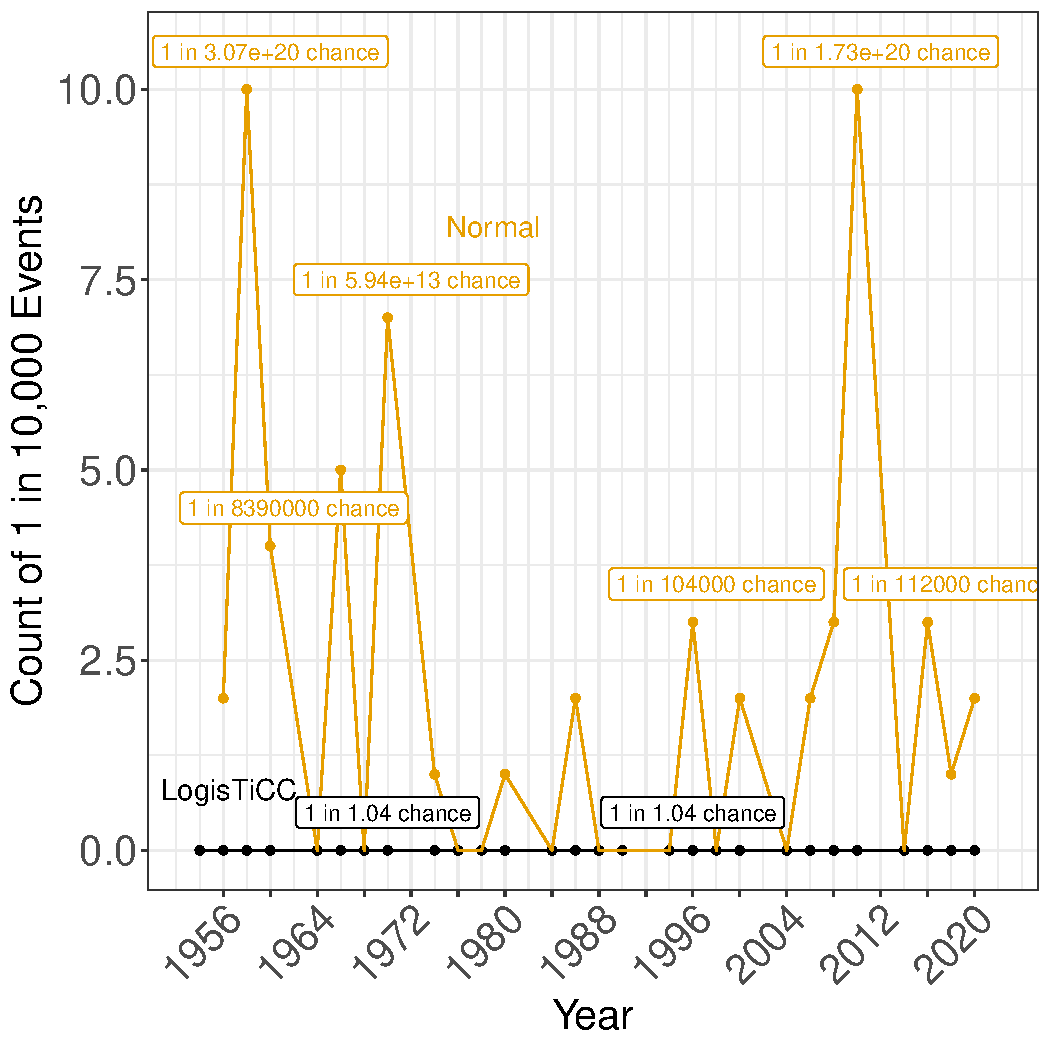
\includegraphics[width=0.7\textwidth]{moralcertitude_oya}
  \caption{Moral Certitude: Count of elections outside a 99.99
    percent credible interval for each election year (with selected points
    labeled with the probability each model gives for seeing this
    many 1-in-10,000 events). Separate calculations appear for the
    normal model (in gold) and our proposed LogisTiCC model (in black).}
  \label{moral}
\end{figure}

\begin{appendices}
\section{Statistical Details}\label{statdetail}

just to show how we can do appendices

This appendix provides the full likelihood function for our model, including all the features described in xxx, as well as situations where the effective vote is both included in the model as a lagged covariate and unobserved (because previous election was uncontested).

To write the full likelihood function, define an uncontestedness indicator $U_{it}$ as 1 if the Democrat runs uncontested, 0 if contested, and $-1$ if the Republican runs uncontested in district $i$ and time $t$.  Then partition elections into four sets depending on whether the current election $i,t$ and its lag $i,t-1$ are contested or uncontested.  Denote
CC as the set of all elections for which $U_{it}=0$ and $U_{i,t-1}=0$;
UC as the set of elections for which $U_{it}\ne 0$ and $U_{i,t-1}= 0$;
CU as the set of elections where $U_{i,t}= 0$ and $U_{i,t-1}\ne 0$;
and UU as the set of elections for which $U_{it}\ne 0$ and $U_{i,t-1}\ne 0$.
Then the likelihood function factors into four parts corresponding to these sets:
\begin{equation}\label{likelihood}
  L = \left(\prod_{i,t\in\{\text{CC}\}} L_{it}^{\text{CC}}\right)
  \left(\prod_{i,t\in\{\text{UC}\}} L_{it}^{\text{UC}}\right)
  \left(\prod_{i,t\in\{\text{CU}\}} L_{it}^{\text{CU}}\right)
  \left(\prod_{i,t\in\{\text{UU}\}} L_{it}^{\text{UU}}\right)
\end{equation}
each of which we now define.

The first component of the likelihood, for when election $i,t$ and $i,t-1$ are both contested, is by far the most prevalent for the US congress.  The likelihood for observation $i,t$ is then simply
\begin{equation}\label{cc}
  L_{it}^{\text{CC}} = \text{ALT}(v_{it}\mid\mu_{it},\phi_t^2,\nu_t).
\end{equation}

The second component of the likelihood accounts for which party is running uncontested at time $t$:
\begin{equation}\label{cu}
  L_{it}^{\text{UC}} = {\bf 1}(U_{it}=1)\psi_{it} + {\bf 1}(U_{it}=-1)(1-\psi_{it}),
\end{equation}
where our censoring assumption from Section \ref{modelU} implies that $\psi_{it}\equiv\int_0^{0.5}\text{ALT}(v^*\mid\mu_{it},\phi_t^2,\nu_t)dv^*$, given the indicator function defined as ${\bf 1}(a)=1$ if $a$ is true and 0 otherwise, for any statement $a$.

To write the third component, where the lagged value of the effective vote is unobserved (because it is uncontested), we require a prior distribution for how this variable is distributed.  The posterior will be computed from the entire model, but to begin we need an assumption about this prior.  One option is to let $v_{i,t-1}^*$ be a censored ALT when unobserved (and equal to $v_{it}$ when observed) but this creates a substantial computational burden with little substantive benefit. Instead, we find we can represent almost all relevant information by assuming that, when unobserved, $v_{i,t-1}^*\sim{\cal N}(Z_{i,t-1}\alpha_t,\sigma_v^2)$, with $Z_{i,t-1}$ a vector of covariates such as lagged presidential vote in a congressional district and incumbency status.  Then this component of the likelihood is
\begin{equation}\label{CU}
  L_{it}^{\text{CU}} = \int_{-\infty}^\infty \text{ALT}(v_{it}\mid\mu_{i,t},\phi_t^2,\nu_t)
  \cdot {\cal N}(v^*\mid Z_{i,t-1}\alpha_t,\sigma_v^2) dv^*,
\end{equation}
where the unobserved lagged effective vote $v^*$ is included in $X$ and so contributes to $\mu_{it}$.

For the final component of the likelihood, we use features of all three previous components, so that
\begin{equation}\label{UU}
  L_{it}^{\text{UU}} = {\bf 1}(U_{it}=1)\psi^\prime_{it} + {\bf 1}(U_{it}=-1)(1-\psi^\prime_{it}),
\end{equation}
where
\begin{equation*}
  \psi^\prime = \int_{-\infty}^\infty\int_0^{0.5}\text{ALT}(v\mid\mu_{i,t},\phi_t^2,\nu_t)dv
  \cdot {\cal N}(v^*\mid Z_{i,t-1}\alpha_t,\sigma_v^2) dv^*.
\end{equation*}



\end{appendices}

\singlespace
\printbibliography
\end{document}

